\documentclass[conference]{IEEEtran}
\usepackage{graphicx}
\usepackage{booktabs}
\usepackage{amsmath}
\usepackage{amssymb}
\usepackage{url}
\usepackage{array}

\title{Benchmarking Off-the-Shelf ASR Systems on Polish Radiology Dictation: Terminology, Numbers, and Clinically Critical Errors}

\author{\IEEEauthorblockN{Konrad Strojny}\IEEEauthorblockA{Affiliation and e-mail to be added before submission}}

\begin{document}
\maketitle

\begin{abstract}
Ready-to-use automatic speech recognition (ASR) systems are increasingly considered for dictating radiology reports, yet their behaviour on Polish clinical speech is poorly characterised. We benchmark 19 off-the-shelf systems (12 open configurations and 7 commercial cloud services) on 939 natural-voice recordings (2.69\,h, 14 speakers) of thyroid ultrasound and head-and-neck radiology. Beyond the word error rate (WER) and character error rate (CER), we measure the correctness of radiology \emph{terminology} (term error rate, TER) against general words (GWER), and errors in numbers, negations, and body side, summarised by a clinically critical error rate (CCER). In classical ASR, radiology terms are recognised 3--6$\times$ worse than general words; large language model (LLM) based transcribers narrow this gap. The best open model (Whisper large-v3) misrecognises 15.8\% of term occurrences but only 3.1\% of general words; the best cloud system (OpenAI gpt-4o-transcribe) reaches WER 5.96\%, and Google Gemini 3.5 Flash has the lowest TER (6.6\%). Number-formatting conventions can inflate raw WER substantially, which is why a number-normalised WER is reported alongside. The higher error rate for terms also persists at equal word frequency, so it is not explained by word rarity alone.
\end{abstract}

\begin{IEEEkeywords}
automatic speech recognition, Polish, radiology, medical dictation, terminology, benchmark
\end{IEEEkeywords}

\section{Introduction}
Radiologists increasingly dictate reports into speech recognition (ASR) systems. General-purpose models such as Whisper perform well on everyday speech, yet in radiology dictation they make more errors on terminology, numbers and units, abbreviations, and proper names. Errors in an imaging report are not equivalent: some are cosmetic (punctuation, inflectional endings), while others change the clinical meaning and may go unnoticed by the physician---a swapped body side (``prawy'' $\to$ ``lewy'', right $\to$ left), a wrong dimension (``45\,mm'' $\to$ ``4\,mm''), a lost negation (``bez zmian'' $\to$ ``zmian'', without changes $\to$ changes), or inserted words that were never spoken (so-called hallucinations).

\noindent\textbf{Research questions.}
\begin{enumerate}
\item How large is the recognition error (WER, CER) on Polish phrases from radiology reports for ready-made ASR solutions: open models run locally and commercial cloud services?
\item How correctly is radiology terminology written (anatomy, image description, diseases and procedures, abbreviations and foreign names) compared with general words in the same recordings? What kinds of errors occur: inflection, word segmentation, misspelling of a heard term, substitution with another word, deletion?
\end{enumerate}

\noindent\textbf{Contributions.}
\begin{itemize}
\item A benchmark of 12 open configurations (10 open models, including language-model variants and a negative control) and 7 commercial cloud services on 939 Polish radiology recordings of natural voice.
\item A term-level error analysis that separates radiology terms (309 forms in four classes) from general words via TER and GWER, and classifies errors into inflection, segmentation, near-miss, substitution, and deletion.
\item Clinically critical error categories (numbers, negations, body side), a pooled clinically critical error rate (CCER), and a proxy for hallucinations (insertions of three or more words).
\item A number-format-normalised WER (WER-N) that separates recognition errors from number-formatting conventions.
\end{itemize}

\section{Related Work}
The open models evaluated here were introduced in prior work: Whisper \cite{r2}, wav2vec 2.0 \cite{r3}, and the multilingual MMS family \cite{r4}. Recent domain-specific and commercial transcribers are documented in their model cards and product documentation (Section~\ref{sec:evaluated}). ASR benchmarking for clinical dictation has largely focused on English and on aggregate word error rates; this study targets Polish radiology dictation and analyses errors at the level of individual terms and clinically critical tokens (numbers, negations, body side).

\section{Data}
\subsection{Research recordings}
The study uses 939 natural-voice Polish radiology recordings (2.69\,h, 14 speakers): short read phrases from thyroid ultrasound and head-and-neck reports, not spontaneous dictation of whole reports. The recordings come from a public research corpus (ADMEDVOICE; Kaggle \texttt{karmarci/polish-medical-multi-source-corpus}, DOI 10.34740/kaggle/ds/6698205, licence CC~BY~4.0) \cite{r1}; only the natural human-voice variant is used.

\subsection{Radiology subset}
Of the eight topical categories of the corpus, the two radiology categories are retained: \texttt{02-001} (thyroid ultrasound) and \texttt{02-003} (head and neck). The test set comprises 939 natural recordings (2.69\,h, 14 speakers, 246 texts). Durations were computed from the WAV headers. Phrases range from 2 to 46 words, 15.8 on average. The same speaker reads the same text several times (129 cases, 258 recordings); no two audio files are identical (MD5), and the metadata were checked for category errors (61 recordings of one speaker were re-assigned from \texttt{02-001} to \texttt{02-003}).

\section{Methods}
\subsection{Study stages}
Each system receives only the recording and the information that the language is Polish. No vocabulary prompts, keyword boosting, custom dictionaries, medical context, or post-recognition correction are used (the ``no-help'' stage). The only exception is Google Gemini (a general LLM), which requires a textual instruction and receives a neutral ``transcribe verbatim'' prompt, with no vocabulary and no mention of medicine.

\subsection{Evaluated systems}\label{sec:evaluated}
\noindent\textbf{Open models (offline).} Whisper medium, large-v3-turbo, and large-v3 \cite{r2}; NVIDIA Canary-1B-v2 \cite{r5}, NVIDIA Parakeet-TDT-0.6B-v3 \cite{r6}, and Qwen3-ASR-1.7B \cite{r8}; NVIDIA FastConformer PL \cite{r7}; wav2vec2 XLSR-53 Polish \cite{r3,r9} and Meta MMS-1b-all \cite{r4}, each without a language model and with a general Polish KenLM \cite{r20}; and Google MedASR \cite{r10}, an English-only model used as a negative control.

\noindent\textbf{Cloud services (online).} OpenAI whisper-1 and gpt-4o-transcribe \cite{r11}, ElevenLabs Scribe v2 \cite{r12}, Deepgram Nova-3 \cite{r13}, AssemblyAI Universal-2 \cite{r14}, Speechmatics (Polish) \cite{r15}, and Google Gemini 3.5 Flash \cite{r16}.

\subsection{Procedure}
The test set is resampled to 16\,kHz mono. Decoding is identical within a model family, without prompts or dictionaries. Whisper uses greedy decoding with \texttt{language=pl}, \texttt{task=transcribe}, fp16 on a Mac GPU (MPS) \cite{r2,r17}. CTC models (wav2vec2, MMS) use greedy decoding; the ``+KenLM'' variants use beam search (pyctcdecode) with a general Polish 5-gram language model from the \texttt{jonatasgrosman/wav2vec2-large-xlsr-53-polish} repository \cite{r9,r19,r20}. NVIDIA NeMo models use their default decoder (Canary with \texttt{source\_lang=target\_lang=pl}). Each cloud recording is sent as a separate request (16\,kHz mono WAV, \texttt{language=pl}) with up to 8 requests in parallel; asynchronous services are polled and their files and jobs removed after reading the transcript.

\subsection{Text normalisation and metrics}
Text normalisation (identical for reference and hypothesis) lowercases, removes punctuation, separates dimensions (``14x12x45'' $\to$ ``14 x 12 x 45''), detaches units (``50mm'' $\to$ ``50 mm''), keeps the decimal comma, and removes technical tokens. Numbers are \emph{not} converted to words.

Metrics are computed with jiwer \cite{r18}: WER and CER with a 95\% confidence interval from bootstrapping over utterances (1{,}000 resamples); WER-N (WER after converting numbers to words with num2words \cite{r23}, ``x''$\to$``na'', and written units to abbreviations); and three clinically critical categories---numbers (tokens with a digit), negations (``nie'', ``bez'', ``brak''), and body side (right/left forms)---as the fraction of misrecognised reference tokens (substitution or deletion). \textbf{CCER} (clinically critical error rate) is a single token-weighted (micro-averaged) rate over the three categories,
\begin{equation}
\mathrm{CCER} = 100\cdot\frac{\text{num\_err}+\text{neg\_err}+\text{side\_err}}{\text{num\_n}+\text{neg\_n}+\text{side\_n}},
\end{equation}
pooled over the 2{,}988 critical reference tokens (1{,}990 numbers, 399 negations, 599 body-side). Each token counts once; only substitutions and deletions count, consistent with the per-category rates. Insertions of $\ge 3$ consecutive words approximate hallucinations. RTF (real-time factor) is processing time divided by audio duration (MacBook Pro M1 Pro, 16\,GB); cloud RTF includes network and queueing and is not directly comparable.

\subsection{Terminology recognition}
The reference vocabulary of the test set has 736 word types without digits, annotated in full against a manual lexicon with one of four classes (Table~\ref{tab:lex}). On the jiwer word alignment, each reference-word occurrence receives one status, checked in order: correct; word segmentation; deletion; inflection (same lemma, different form; hypothesis lemmas from simplemma \cite{r22}); near-miss (character Levenshtein distance $\le \max(1, \mathrm{round}(0.3\cdot\text{length}))$, unless a meaning-bearing prefix changes, which counts as a substitution); substitution. TER is the fraction of term occurrences not \emph{correct}; TER-L counts only near-miss, substitution, and deletion; GWER is the same rate for general words; the ratio TER/GWER indicates how many times harder terms are. Error rates are also computed in bins of general-Polish word frequency (Zipf scale; wordfreq \cite{r21,r24}).

\section{Results}
\subsection{Open models}
Table~\ref{tab:wer-open} reports WER and the clinical categories. Whisper large-v3 is the best open model (WER 8.03\%), also relative to the newer 2025--2026 models. CCER confirms the ranking but exposes clinically risky outliers: Whisper large-v3 has the lowest CCER among open models (2.71\%), close to its three category rates; Qwen3-ASR reaches a much higher CCER (9.27\%) than its low number-error rate (7.7\%) because of frequent negation (10.3\%) and body-side (13.7\%) errors. The new NVIDIA models lose mainly on number formatting (20--26\% on dimensions); after normalising the format (WER-N 14--15\%) they approach Whisper medium. A general Polish language model improves the CTC models (wav2vec2 58.3$\to$52.8\%, MMS 35.2$\to$32.1\%). FastConformer PL confuses body side in 37\% of cases. MedASR, English-only, gives WER $\sim$100\%, replacing Polish speech with English medical terms.

\begin{table*}[t]
\centering
\caption{Open models (offline). Values in percent; WER with 95\% CI. Numbers, Negations, Body side: fraction of misrecognised tokens in that category (n = 1,990/399/599); CCER pools the three over 2,988 tokens.}
\label{tab:wer-open}
\resizebox{\textwidth}{!}{%
\begin{tabular}{lcccccccccc}
\toprule
Model & WER [95\% CI] & WER-N & CER & Numbers & Negations & Body side & CCER & Ins.$\ge$3 & RTF \\
\midrule
Whisper large-v3 & 8.03 [7.43--8.73] & 7.61 & 2.17 & 2.8 & 2.8 & 2.5 & 2.71 & 2 & 0.139 \\
Whisper large-v3-turbo & 9.75 [9.1--10.44] & 9.21 & 2.57 & 2.8 & 1.5 & 2.8 & 2.61 & 3 & 0.082 \\
Whisper medium & 13.77 [12.94--14.64] & 13.12 & 3.94 & 4.1 & 2.5 & 3.8 & 3.85 & 6 & 0.071 \\
NVIDIA Parakeet-TDT-0.6B-v3 & 18.21 [17.2--19.2] & 15.03 & 6.29 & 20.8 & 1.8 & 5.3 & 15.13 & 3 & 0.097 \\
NVIDIA Canary-1B-v2 & 20.05 [18.95--21.34] & 14.04 & 8.66 & 25.6 & 1.5 & 5.0 & 18.27 & 8 & 0.295 \\
Qwen3-ASR-1.7B & 21.8 [20.9--22.76] & 18.35 & 7.37 & 7.7 & 10.3 & 13.7 & 9.27 & 3 & 0.151 \\
Meta MMS-1b-all (pol) + KenLM & 32.07 [30.88--33.35] & 25.72 & 12.47 & 81.8 & 1.8 & 6.8 & 56.09 & 13 & 0.101 \\
Meta MMS-1b-all (pol adapter, no LM) & 35.22 [33.87--36.48] & 27.46 & 13.17 & 57.3 & 6.3 & 11.0 & 41.23 & 36 & 0.088 \\
NVIDIA FastConformer PL (hybrid, P\&C) & 50.7 [49.26--52.17] & 31.4 & 30.29 & 100.0 & 7.5 & 37.1 & 75.03 & 41 & 0.03 \\
wav2vec2 XLSR-53 Polish + KenLM & 52.8 [51.22--54.3] & 32.94 & 29.54 & 100.0 & 14.0 & 20.7 & 72.62 & 132 & 0.066 \\
wav2vec2 XLSR-53 Polish (no LM) & 58.31 [56.67--59.69] & 41.08 & 30.68 & 100.0 & 23.8 & 25.5 & 74.90 & 121 & 0.07 \\
Google MedASR & 99.65 [99.21--100.08] & 99.01 & 80.48 & 98.2 & 100.0 & 100.0 & 98.83 & 41 & 0.011 \\
\bottomrule
\end{tabular}}
\end{table*}

\subsection{Cloud services}
Table~\ref{tab:wer-cloud} reports the cloud services. OpenAI gpt-4o-transcribe is the best system overall (WER 5.96\%, CER 2.03\%, WER-N 4.47\%, lowest number-error rate 1.9\%); 54\% of its utterances are error-free. Gemini 3.5 Flash writes terms best (TER 6.6\%) and has the best WER-N (4.18\%) and fewest negation errors (1.0\%), at the cost of a higher raw WER from ``smoothing''. By CCER, gpt-4o-transcribe is the clinically safest (2.07\%) and Gemini 3.5 Flash is close (2.74\%), whereas ElevenLabs Scribe v2 has the highest CCER among cloud services (65.56\%): it spells numbers out (``2\,mm'' $\to$ ``dw\'och milimetr\'ow''), which inflates raw WER to 28.27\% (WER-N 5.22\%) and makes numbers a critical-error source although its TER is low.

\begin{table*}[t]
\centering
\caption{Cloud services (online). Columns as in Table~\ref{tab:wer-open}; RTF includes network and queueing and is not comparable with local models.}
\label{tab:wer-cloud}
\resizebox{\textwidth}{!}{%
\begin{tabular}{lcccccccccc}
\toprule
Model & WER [95\% CI] & WER-N & CER & Numbers & Negations & Body side & CCER & Ins.$\ge$3 & RTF \\
\midrule
OpenAI gpt-4o-transcribe & 5.96 [5.4--6.52] & 4.47 & 2.03 & 1.9 & 2.0 & 2.7 & 2.07 & 1 & 0.021 \\
OpenAI whisper-1 & 9.93 [9.26--10.62] & 9.45 & 2.58 & 3.5 & 3.3 & 3.5 & 3.48 & 1 & 0.032 \\
AssemblyAI Universal-2 & 10.25 [9.54--10.96] & 9.71 & 2.77 & 3.5 & 2.8 & 3.8 & 3.48 & 1 & 0.265 \\
Google Gemini 3.5 Flash & 10.4 [9.75--11.09] & 4.18 & 4.03 & 3.0 & 1.0 & 3.0 & 2.74 & 8 & 0.076 \\
Deepgram Nova-3 & 15.06 [14.3--15.84] & 8.48 & 7.88 & 8.0 & 3.5 & 2.5 & 6.33 & 6 & 0.018 \\
Speechmatics (pl) & 19.41 [18.68--20.18] & 16.37 & 6.18 & 16.1 & 0.3 & 7.0 & 12.18 & 1 & 0.03 \\
ElevenLabs Scribe v2 & 28.27 [26.22--30.33] & 5.22 & 23.53 & 97.7 & 1.3 & 1.7 & 65.56 & 65 & 0.037 \\
\bottomrule
\end{tabular}}
\end{table*}

\subsection{Radiology terminology}
Table~\ref{tab:ter-open} and Table~\ref{tab:ter-cloud} give TER and its decomposition. Terms are 3.4--5.7$\times$ harder than general words for the classical models with GWER $\le$ 10.2\%. Near-miss dominates: for Whisper large-v3, 8.7 of the 15.8 percentage points of TER are near-misses (``TIRADS''$\to$``TIRAC''/``TIRATS''/``TIRAS'', 104 of 176 occurrences; ``color''$\to$``kolor''; ``mi\k{a}\.{z}sz''$\to$``miosz''), i.e., the model hears the term but does not know its spelling. Abbreviations and foreign names are the hardest class (Table~\ref{tab:class}). The exception is ElevenLabs Scribe v2, for which terms are easier than general words (TER/GWER 0.7, the only system below 1.0). The domain effect is not reducible to word rarity: at equal general frequency (Zipf 3--5) terms still have 10--13\% errors versus 2--3\% for general words (Fig.~\ref{fig:zipf}).

\begin{table*}[t]
\centering
\caption{Open models: radiology terminology. Values in percent; the columns Inflection\,\ldots\,Deletion give the fraction of all term occurrences (n = 5,429); their sum is TER.}
\label{tab:ter-open}
\resizebox{\textwidth}{!}{%
\begin{tabular}{lccccccccc}
\toprule
Model & TER [95\% CI] & TER-L & GWER & TER/GWER & Inflection & Segm. & Near-miss & Substitution & Deletion \\
\midrule
Whisper large-v3 & 15.8 [14.8--17.1] & 13.0 & 3.1 & 5.1 & 0.9 & 2.0 & 8.7 & 3.4 & 0.8 \\
Whisper large-v3-turbo & 19.5 [18.4--20.8] & 16.5 & 3.4 & 5.7 & 1.1 & 1.9 & 11.4 & 4.1 & 1.0 \\
Whisper medium & 27.0 [25.6--28.4] & 23.6 & 5.6 & 4.8 & 1.3 & 2.1 & 15.1 & 7.2 & 1.3 \\
NVIDIA Parakeet-TDT-0.6B-v3 & 28.9 [27.6--30.3] & 25.3 & 5.9 & 4.9 & 1.0 & 2.7 & 14.9 & 7.4 & 3.0 \\
NVIDIA Canary-1B-v2 & 30.1 [28.8--31.4] & 26.3 & 5.7 & 5.3 & 1.5 & 2.3 & 14.5 & 10.0 & 1.8 \\
Meta MMS-1b-all (pol) + KenLM & 30.3 [28.9--31.5] & 24.1 & 9.0 & 3.4 & 1.5 & 4.8 & 14.8 & 7.0 & 2.2 \\
Meta MMS-1b-all (no LM) & 39.3 [37.8--40.7] & 35.3 & 14.1 & 2.8 & 1.2 & 2.8 & 24.2 & 8.0 & 3.0 \\
Qwen3-ASR-1.7B & 39.3 [37.7--40.7] & 33.9 & 10.2 & 3.8 & 3.0 & 2.3 & 20.1 & 10.8 & 3.0 \\
wav2vec2 XLSR-53 Polish + KenLM & 46.0 [44.5--47.4] & 40.0 & 26.0 & 1.8 & 1.6 & 4.4 & 18.4 & 18.7 & 2.9 \\
NVIDIA FastConformer PL & 53.9 [52.3--55.3] & 49.2 & 23.2 & 2.3 & 1.7 & 3.0 & 22.4 & 20.7 & 6.1 \\
wav2vec2 XLSR-53 Polish (no LM) & 54.9 [53.3--56.3] & 49.7 & 31.9 & 1.7 & 1.6 & 3.7 & 22.9 & 22.4 & 4.4 \\
Google MedASR (neg. control) & 97.6 [97.2--98.1] & 97.6 & 98.1 & 1.0 & 0.0 & 0.0 & 0.5 & 50.1 & 47.1 \\
\bottomrule
\end{tabular}}
\end{table*}

\begin{table*}[t]
\centering
\caption{Cloud services: radiology terminology (same columns as Table~\ref{tab:ter-open}).}
\label{tab:ter-cloud}
\resizebox{0.8\textwidth}{!}{%
\begin{tabular}{lccccccccc}
\toprule
Model & TER [95\% CI] & TER-L & GWER & TER/GWER & Inflection & Segm. & Near-miss & Substitution & Deletion \\
\midrule
Google Gemini 3.5 Flash & 6.6 [5.8--7.4] & 4.8 & 4.0 & 1.6 & 1.3 & 0.4 & 2.8 & 1.6 & 0.5 \\
ElevenLabs Scribe v2 & 7.2 [6.4--8.1] & 5.7 & 10.1 & 0.7 & 0.6 & 0.9 & 3.7 & 1.6 & 0.4 \\
OpenAI gpt-4o-transcribe & 7.6 [6.8--8.5] & 4.5 & 2.9 & 2.6 & 1.4 & 1.7 & 1.8 & 2.2 & 0.5 \\
Deepgram Nova-3 & 16.6 [15.3--17.9] & 13.9 & 11.1 & 1.5 & 1.2 & 1.5 & 7.6 & 4.4 & 1.9 \\
OpenAI whisper-1 & 19.1 [17.9--20.3] & 15.5 & 3.7 & 5.2 & 1.3 & 2.3 & 9.8 & 4.7 & 0.9 \\
AssemblyAI Universal-2 & 19.3 [18.0--20.6] & 15.8 & 4.3 & 4.5 & 1.1 & 2.4 & 9.8 & 4.9 & 1.1 \\
Speechmatics (pl) & 29.2 [27.9--30.4] & 23.0 & 6.7 & 4.4 & 2.4 & 3.8 & 11.4 & 10.1 & 1.6 \\
\bottomrule
\end{tabular}}
\end{table*}

\begin{table}[t]
\centering
\caption{Term lexicon by class (reference set).}
\label{tab:lex}
\begin{tabular}{lrrr}
\toprule
Class & Forms & Lemmas & Occurrences \\
\midrule
Anatomy & 112 & 68 & 2,326 \\
Image description & 114 & 59 & 2,142 \\
Pathology/procedures & 54 & 35 & 410 \\
Abbreviations/foreign & 29 & 29 & 551 \\
\textbf{Terms total} & \textbf{309} & \textbf{191} & \textbf{5,429} \\
General words & 424 & 319 & 9,405 \\
\bottomrule
\end{tabular}
\end{table}

\begin{table}[t]
\centering
\caption{TER by term class (selected models).}
\label{tab:class}
\begin{tabular}{lcccc}
\toprule
Model & Anatomy & Image & Pathology & Abbrev. \\
\midrule
Whisper large-v3 & 12.2 & 12.6 & 15.9 & 43.9 \\
Whisper large-v3-turbo & 13.5 & 17.4 & 15.1 & 56.8 \\
Parakeet-TDT-0.6B-v3 & 23.3 & 24.0 & 33.4 & 68.2 \\
Canary-1B-v2 & 27.7 & 23.7 & 33.4 & 62.4 \\
Qwen3-ASR-1.7B & 30.0 & 40.6 & 58.1 & 59.4 \\
\bottomrule
\end{tabular}
\end{table}

\begin{figure*}[t]
\centering
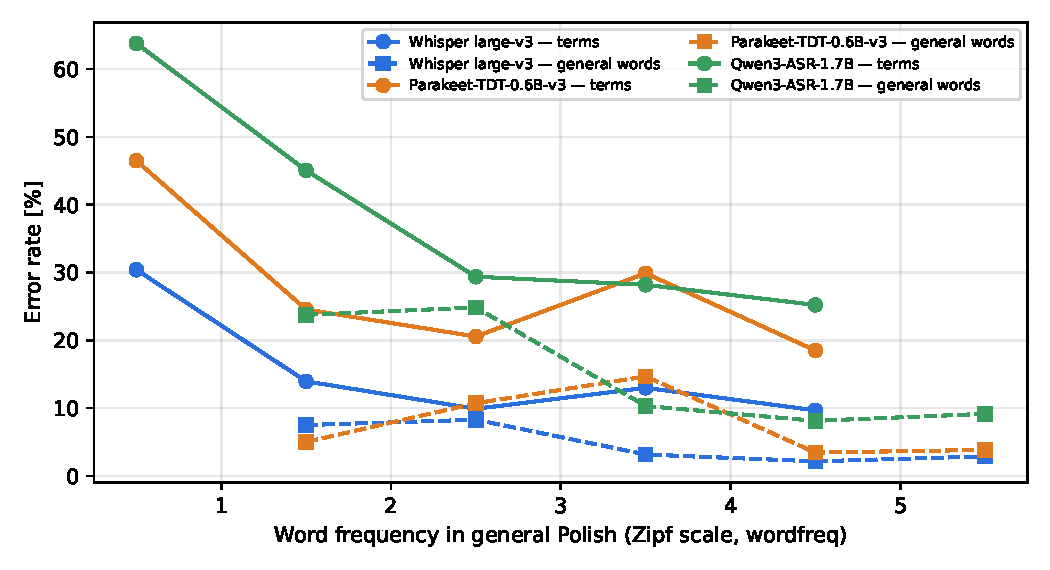
\includegraphics[width=0.78\textwidth]{fig_terms_vs_freq.pdf}
\caption{Error rate versus word frequency in general Polish (Zipf scale) for terms and general words, for three representative models. At equal frequency, terms are still markedly harder.}
\label{fig:zipf}
\end{figure*}

\section{Discussion}
\noindent\textbf{Classical ASR versus LLM-based transcribers.} The results separate two families. Classical acoustic ASR systems treat terminology as an out-of-vocabulary problem: the signal is recognised, but the term is written as a phonetically plausible near-miss, which is why TER/GWER is high and near-miss dominates. LLM-based transcribers (gpt-4o-transcribe, Gemini 3.5 Flash, and, in WER-N terms, ElevenLabs) bring lexical knowledge to spelling and narrow the gap. The trade-off is a tendency to ``smooth'' the output (punctuation, word segmentation, insertions), which raw WER penalises but which a clinician may tolerate. A number-normalised WER and TER therefore give a more faithful picture of clinical usefulness than aggregate WER alone.

\noindent\textbf{Number verbalisation is a metric artefact.} ElevenLabs renders numbers as words, producing a raw WER of 28.27\% that would wrongly suggest a poor system; its WER-N of 5.22\% places it among the best. Benchmarks of morphologically rich radiology dictation should report a number-normalised metric and state which convention (digits versus words) the deployment requires.

\noindent\textbf{What matters clinically is not aggregate WER.} The critical categories diverge from the aggregate ranking, and CCER summarises them: gpt-4o-transcribe leads (2.07\%), Gemini 3.5 Flash follows (2.74\%), and ElevenLabs is the riskiest among cloud services (65.56\%). Model selection and human review should target numbers, negations, and body side explicitly.

\noindent\textbf{Near-miss dominance points to a cheap remedy.} Because most terminology errors are near-misses, a lexicon-driven post-correction or a decoding-time term list could remove a large share of errors without retraining---an upper bound is the gap between TER (15.8\%) and TER-L (13.0\%) for Whisper large-v3.

\section{Limitations}
The test set is small (2.69\,h), covers two categories dominated by thyroid ultrasound, and consists of read phrases rather than spontaneous dictation, so results may not transfer to full free-form reports or other regions. The term annotation was produced by a language model and not verified by a radiologist; the term/general boundary is conventional. Near-miss classification uses an arbitrary edit-distance threshold, and raw WER penalises benign formatting differences (hence WER-N and TER). Local RTF was measured on one machine; cloud RTF is not directly comparable. Several planned systems could not be evaluated: Cohere Transcribe 03-2026 and NVIDIA Nemotron 3.5 Transcribe (gated or requiring a rented GPU), Soniox (no account balance), Google Chirp (requires a Google Cloud project), and Azure AI Speech (no key). The dedicated Google transcription model \texttt{gemini-3.5-transcribe} enforces a limit of 100 requests per day on its first tier, which precludes a full run in one day; the general \texttt{gemini-3.5-flash} model was measured instead. Our study measures systems without support (no vocabulary prompts or post-correction); the effect of such support is future work.

\section{Conclusion}
Ready-made ASR systems are close to usable for Polish radiology dictation, but aggregate WER hides the clinically relevant failures. On 939 natural-voice recordings, the best open model (Whisper large-v3) reaches WER 8.03\% but misrecognises 15.8\% of radiology terms, 3--6$\times$ more than general words, with near-misses dominating. LLM-based transcribers narrow this gap: OpenAI gpt-4o-transcribe attains the best overall WER (5.96\%) and CCER (2.07\%), and Google Gemini 3.5 Flash the best terminology accuracy (TER 6.6\%). Number formatting can inflate raw WER dramatically, so a number-normalised metric is essential; ElevenLabs Scribe v2 drops from 28.27\% raw WER to 5.22\% WER-N. Because errors concentrate in numbers, negations, body side, and a handful of abbreviations, both model selection and quality assurance should target these tokens rather than the aggregate score, and a lexicon-based post-correction is a promising, low-cost next step.

\section*{Data and Code Availability}
The ADMEDVOICE corpus is public (Kaggle \texttt{karmarci/polish-medical-multi-source-corpus}, DOI 10.34740/kaggle/ds/6698205, licence CC~BY~4.0) \cite{r1}. The evaluation code, the term lexicon, and the per-system transcriptions and metrics are provided in the project repository (\url{https://github.com/kocasp/halucination_research}); the audio is not redistributed and is reconstructed from ADMEDVOICE with \texttt{scripts/build\_radiology\_db.py}.

\section*{Reproducibility}
Offline inference used PyTorch 2.15 (MPS), transformers 5.23 (Qwen3-ASR in a separate environment), NVIDIA NeMo 3.0, and qwen-asr; metrics used jiwer, pyctcdecode 0.5 with KenLM, num2words, wordfreq 3.1.1, and simplemma 2.0. The term analysis is reproduced with \texttt{uv run python terms.py} (Section~V-C). All runs used a MacBook Pro M1 Pro (16\,GB) for local models.

\begin{thebibliography}{99}
\bibitem{r1} A. Czy\.zewski et al., ``A Comprehensive Polish Medical Speech Dataset for Enhancing Automatic Medical Dictation,'' \emph{Scientific Data}, vol. 12, art. 1436, 2025. doi:10.1038/s41597-025-05776-1.
\bibitem{r2} A. Radford, J. W. Kim, T. Xu, G. Brockman, C. McLeavey, and I. Sutskever, ``Robust Speech Recognition via Large-Scale Weak Supervision,'' in \emph{Proc. ICML}, 2023. arXiv:2212.04356.
\bibitem{r3} A. Baevski, Y. Zhou, A. Mohamed, and M. Auli, ``wav2vec 2.0: A Framework for Self-Supervised Learning of Speech Representations,'' in \emph{Proc. NeurIPS}, 2020. arXiv:2006.11477.
\bibitem{r4} V. Pratap, A. Tjandra, B. Shi, et al., ``Scaling Speech Technology to 1,000+ Languages,'' 2023. arXiv:2305.13516.
\bibitem{r5} NVIDIA, ``Canary-1B-v2 model card,'' Hugging Face, 2025. \url{https://huggingface.co/nvidia/canary-1b-v2}
\bibitem{r6} NVIDIA, ``Parakeet-TDT-0.6B-v3 model card,'' Hugging Face, 2025. \url{https://huggingface.co/nvidia/parakeet-tdt-0.6b-v3}
\bibitem{r7} NVIDIA, ``Polish FastConformer hybrid (P\&C) model card,'' Hugging Face. \url{https://huggingface.co/nvidia/stt_pl_fastconformer_hybrid_large_pc}
\bibitem{r8} Qwen Team, ``Qwen3-ASR-1.7B model card,'' Hugging Face, 2026. \url{https://huggingface.co/Qwen/Qwen3-ASR-1.7B}
\bibitem{r9} J. Grosman, ``wav2vec2-large-xlsr-53-polish model card,'' Hugging Face. \url{https://huggingface.co/jonatasgrosman/wav2vec2-large-xlsr-53-polish}
\bibitem{r10} Google, ``MedASR model card,'' Hugging Face. \url{https://huggingface.co/google/medasr}
\bibitem{r11} OpenAI, ``Audio transcription API (whisper-1, gpt-4o-transcribe),'' Documentation, 2026. \url{https://platform.openai.com/docs}
\bibitem{r12} ElevenLabs, ``Speech-to-text (Scribe) documentation,'' 2026. \url{https://elevenlabs.io/docs}
\bibitem{r13} Deepgram, ``Nova-3 documentation,'' 2026. \url{https://developers.deepgram.com}
\bibitem{r14} AssemblyAI, ``Documentation,'' 2026. \url{https://www.assemblyai.com/docs}
\bibitem{r15} Speechmatics, ``Documentation,'' 2026. \url{https://docs.speechmatics.com}
\bibitem{r16} Google, ``Gemini API documentation,'' 2026. \url{https://ai.google.dev/gemini-api/docs}
\bibitem{r17} T. Wolf, L. Debut, V. Sanh, et al., ``Transformers: State-of-the-Art Natural Language Processing,'' in \emph{Proc. EMNLP (system demonstrations)}, 2020. arXiv:1910.03771.
\bibitem{r18} A. C. Morris, V. Maier, and P. Green, ``jiwer: Evaluate ASR output,'' GitHub. \url{https://github.com/jitsi/jiwer}
\bibitem{r19} Kensho Technologies, ``pyctcdecode,'' GitHub. \url{https://github.com/kensho-technologies/pyctcdecode}
\bibitem{r20} K. Heafield, ``KenLM: Faster and Smaller Language Model Queries,'' in \emph{Proc. WMT}, 2011.
\bibitem{r21} R. Speer, J. Chin, and A. Lin, ``wordfreq,'' GitHub, 2018. \url{https://github.com/rspeer/wordfreq}
\bibitem{r22} A. Barbaresi, ``simplemma,'' GitHub. \url{https://github.com/adbar/simplemma}
\bibitem{r23} Savoir-faire Linux, ``num2words,'' GitHub. \url{https://github.com/savoirfairelinux/num2words}
\bibitem{r24} G. K. Zipf, \emph{Human Behavior and the Principle of Least Effort}. Addison-Wesley, 1949.
\end{thebibliography}

\end{document}
